\documentclass{standalone}
\usepackage{tikz}
\usetikzlibrary{patterns, positioning}
\usetikzlibrary{shapes.misc}
\usepackage[outline]{contour}
\contourlength{1.5pt} 


\begin{document}
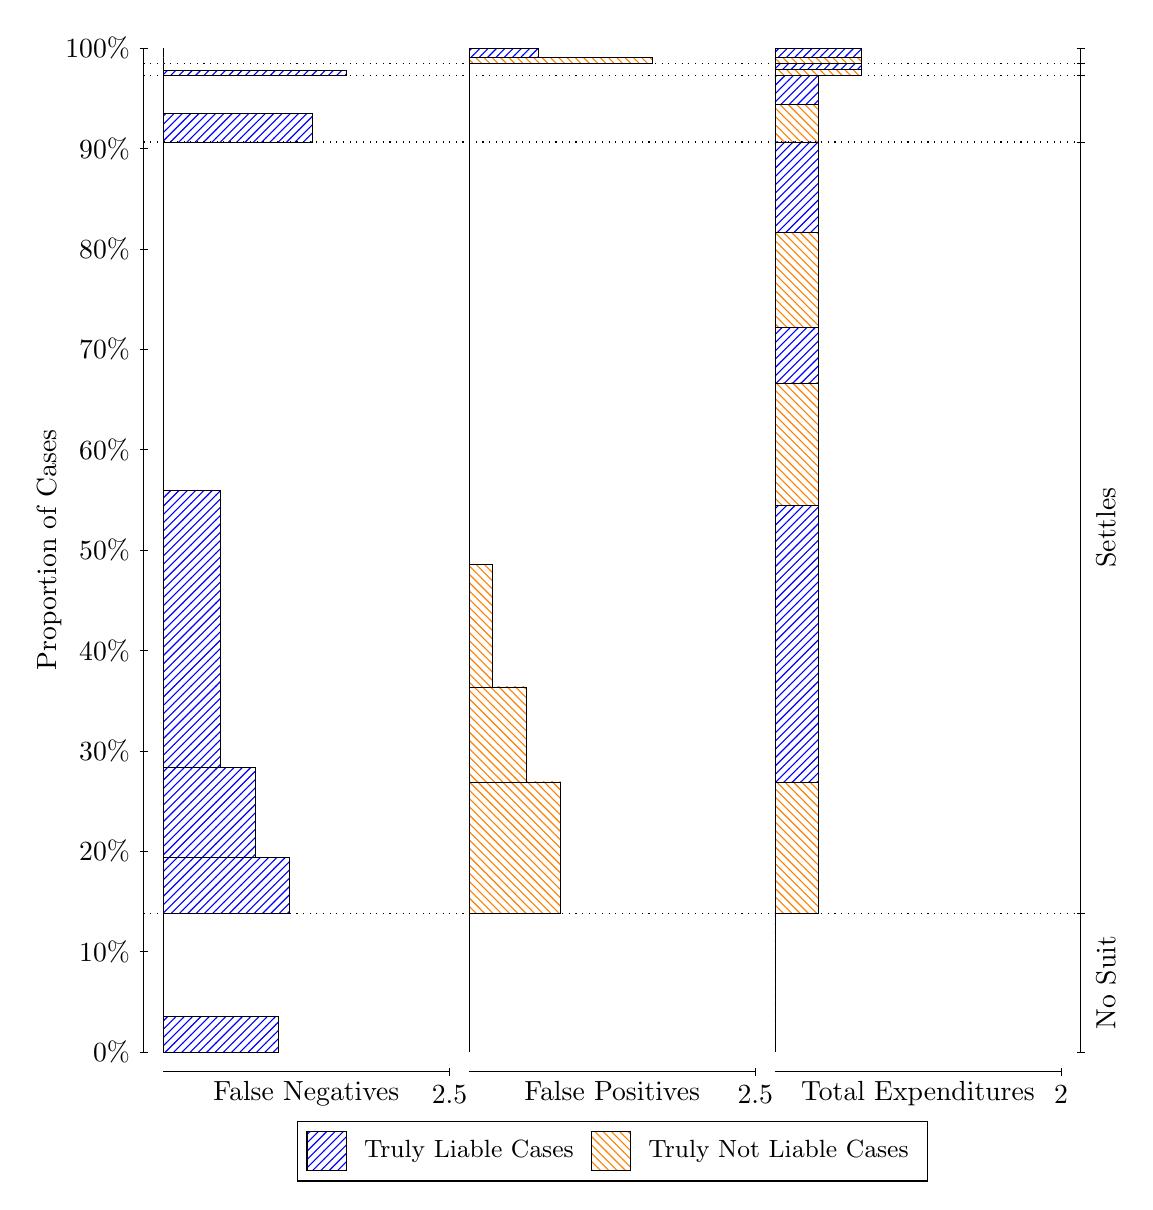
\begin{tikzpicture}
\draw[black, very thin] (1.5,1.75) -- (1.5,14.5);
\node[rotate=90, text=black, anchor=center] at (0.3, 8.125) {Proportion of Cases};
\draw[black, very thin] (1.45,1.75) -- (1.55,1.75);
\node[text=black, anchor=east] at (1.45, 1.75) {0\%};
\draw[black, very thin] (1.45,3.025) -- (1.55,3.025);
\node[text=black, anchor=east] at (1.45, 3.025) {10\%};
\draw[black, very thin] (1.45,4.3) -- (1.55,4.3);
\node[text=black, anchor=east] at (1.45, 4.3) {20\%};
\draw[black, very thin] (1.45,5.575) -- (1.55,5.575);
\node[text=black, anchor=east] at (1.45, 5.575) {30\%};
\draw[black, very thin] (1.45,6.85) -- (1.55,6.85);
\node[text=black, anchor=east] at (1.45, 6.85) {40\%};
\draw[black, very thin] (1.45,8.125) -- (1.55,8.125);
\node[text=black, anchor=east] at (1.45, 8.125) {50\%};
\draw[black, very thin] (1.45,9.4) -- (1.55,9.4);
\node[text=black, anchor=east] at (1.45, 9.4) {60\%};
\draw[black, very thin] (1.45,10.675) -- (1.55,10.675);
\node[text=black, anchor=east] at (1.45, 10.675) {70\%};
\draw[black, very thin] (1.45,11.95) -- (1.55,11.95);
\node[text=black, anchor=east] at (1.45, 11.95) {80\%};
\draw[black, very thin] (1.45,13.225) -- (1.55,13.225);
\node[text=black, anchor=east] at (1.45, 13.225) {90\%};
\draw[black, very thin] (1.45,14.5) -- (1.55,14.5);
\node[text=black, anchor=east] at (1.45, 14.5) {100\%};

\draw[black, very thin] (13.4,1.75) -- (13.4,14.5);
\draw[black, very thin] (13.35,1.75) -- (13.45,1.75);
\node[anchor=west] at (13.35, 1.75) {};
\draw[black, very thin] (13.35,3.5135) -- (13.45,3.5135);
\node[anchor=west] at (13.35, 3.5135) {};
\draw[black, very thin] (13.35,13.307) -- (13.45,13.307);
\node[anchor=west] at (13.35, 13.307) {};
\draw[black, very thin] (13.35,14.149) -- (13.45,14.149);
\node[anchor=west] at (13.35, 14.149) {};
\draw[black, very thin] (13.35,14.303) -- (13.45,14.303);
\node[anchor=west] at (13.35, 14.303) {};
\draw[black, very thin] (13.35,14.5) -- (13.45,14.5);
\node[anchor=west] at (13.35, 14.5) {};

\draw[black, very thin, pattern color=blue, pattern=north east lines] (1.75,1.75) rectangle (3.2033,2.2065);
\draw[black, very thin, pattern color=orange, pattern=north west lines] (1.75,2.2065) rectangle (1.75,3.5135);
\draw[black, very thin, pattern color=blue, pattern=north east lines] (1.75,3.5135) rectangle (3.3487,4.2175);
\draw[black, very thin, pattern color=blue, pattern=north east lines] (1.75,4.2175) rectangle (2.9127,5.3671);
\draw[black, very thin, pattern color=blue, pattern=north east lines] (1.75,5.3671) rectangle (2.4767,8.8817);
\draw[black, very thin, pattern color=orange, pattern=north west lines] (1.75,8.8817) rectangle (1.75,13.307);
\draw[black, very thin, pattern color=blue, pattern=north east lines] (1.75,13.307) rectangle (3.6393,13.669);
\draw[black, very thin, pattern color=orange, pattern=north west lines] (1.75,13.669) rectangle (1.75,14.149);
\draw[black, very thin, pattern color=blue, pattern=north east lines] (1.75,14.149) rectangle (4.0753,14.22);
\draw[black, very thin, pattern color=orange, pattern=north west lines] (1.75,14.22) rectangle (1.75,14.303);
\draw[black, very thin, pattern color=orange, pattern=north west lines] (1.75,14.303) rectangle (1.75,14.382);
\draw[black, very thin, pattern color=blue, pattern=north east lines] (1.75,14.382) rectangle (1.75,14.5);
\draw[black, very thin, pattern color=orange, pattern=north west lines] (5.6333,1.75) rectangle (5.6333,3.057);
\draw[black, very thin, pattern color=blue, pattern=north east lines] (5.6333,3.057) rectangle (5.6333,3.5135);
\draw[black, very thin, pattern color=orange, pattern=north west lines] (5.6333,3.5135) rectangle (6.796,5.1811);
\draw[black, very thin, pattern color=orange, pattern=north west lines] (5.6333,5.1811) rectangle (6.36,6.3867);
\draw[black, very thin, pattern color=orange, pattern=north west lines] (5.6333,6.3867) rectangle (5.924,7.9392);
\draw[black, very thin, pattern color=blue, pattern=north east lines] (5.6333,7.9392) rectangle (5.6333,13.307);
\draw[black, very thin, pattern color=orange, pattern=north west lines] (5.6333,13.307) rectangle (5.6333,13.788);
\draw[black, very thin, pattern color=blue, pattern=north east lines] (5.6333,13.788) rectangle (5.6333,14.149);
\draw[black, very thin, pattern color=orange, pattern=north west lines] (5.6333,14.149) rectangle (5.6333,14.232);
\draw[black, very thin, pattern color=blue, pattern=north east lines] (5.6333,14.232) rectangle (5.6333,14.303);
\draw[black, very thin, pattern color=orange, pattern=north west lines] (5.6333,14.303) rectangle (7.9587,14.382);
\draw[black, very thin, pattern color=blue, pattern=north east lines] (5.6333,14.382) rectangle (6.5053,14.5);
\draw[black, very thin, pattern color=orange, pattern=north west lines] (9.5167,1.75) rectangle (9.5167,3.057);
\draw[black, very thin, pattern color=blue, pattern=north east lines] (9.5167,3.057) rectangle (9.5167,3.5135);
\draw[black, very thin, pattern color=orange, pattern=north west lines] (9.5167,3.5135) rectangle (10.062,5.1811);
\draw[black, very thin, pattern color=blue, pattern=north east lines] (9.5167,5.1811) rectangle (10.062,8.6958);
\draw[black, very thin, pattern color=orange, pattern=north west lines] (9.5167,8.6958) rectangle (10.062,10.248);
\draw[black, very thin, pattern color=blue, pattern=north east lines] (9.5167,10.248) rectangle (10.062,10.952);
\draw[black, very thin, pattern color=orange, pattern=north west lines] (9.5167,10.952) rectangle (10.062,12.158);
\draw[black, very thin, pattern color=blue, pattern=north east lines] (9.5167,12.158) rectangle (10.062,13.307);
\draw[black, very thin, pattern color=orange, pattern=north west lines] (9.5167,13.307) rectangle (10.062,13.788);
\draw[black, very thin, pattern color=blue, pattern=north east lines] (9.5167,13.788) rectangle (10.062,14.149);
\draw[black, very thin, pattern color=orange, pattern=north west lines] (9.5167,14.149) rectangle (10.607,14.232);
\draw[black, very thin, pattern color=blue, pattern=north east lines] (9.5167,14.232) rectangle (10.607,14.303);
\draw[black, very thin, pattern color=orange, pattern=north west lines] (9.5167,14.303) rectangle (10.607,14.382);
\draw[black, very thin, pattern color=blue, pattern=north east lines] (9.5167,14.382) rectangle (10.607,14.5);
\draw[black, dotted] (1.5,3.5135) -- (13.4,3.5135);
\draw[black, dotted] (1.5,13.307) -- (13.4,13.307);
\draw[black, dotted] (1.5,14.149) -- (13.4,14.149);
\draw[black, dotted] (1.5,14.303) -- (13.4,14.303);
\draw[black, very thin] (1.75,1.5) -- (5.3833,1.5);
\node[text=black, anchor=north] at (3.5667, 1.5) {False Negatives};
\draw[black, very thin] (5.3833,1.45) -- (5.3833,1.55);
\node[text=black, anchor=north] at (5.3833, 1.45) {2.5};

\draw[black, very thin] (5.6333,1.5) -- (9.2667,1.5);
\node[text=black, anchor=north] at (7.45, 1.5) {False Positives};
\draw[black, very thin] (9.2667,1.45) -- (9.2667,1.55);
\node[text=black, anchor=north] at (9.2667, 1.45) {2.5};

\draw[black, very thin] (9.5167,1.5) -- (13.15,1.5);
\node[text=black, anchor=north] at (11.333, 1.5) {Total Expenditures};
\draw[black, very thin] (13.15,1.45) -- (13.15,1.55);
\node[text=black, anchor=north] at (13.15, 1.45) {2};

\node[text=black, centered, rotate=90] at (13.72, 2.6317) {\contour{white}{No Suit}};
\node[text=black, centered, rotate=90] at (13.72, 8.4105) {\contour{white}{Settles}};




\draw (7.449999999999999,1.5) node[draw=none] (baseCoordinate) {};
\begin{scope}[align=center]
        \matrix[scale=0.5, draw=black, below=0.5cm of baseCoordinate, nodes={draw}, column sep=0.1cm]{
            \node[rectangle, draw, minimum width=0.5cm, minimum height=0.5cm, pattern color=blue, pattern=north east lines] {}; &
            \node[draw=none, font=\small, text=black] (B) {Truly Liable Cases}; &
            \node[rectangle, draw, minimum width=0.5cm, minimum height=0.5cm, pattern color=orange, pattern=north west lines] {}; &
            \node[draw=none, font=\small, text=black] (B) {Truly Not Liable Cases}; \\
            };
\end{scope}

\end{tikzpicture}
\end{document}